\section{Funciones Integrables}
Hasta ahora no hemos hecho más que definir la integral y las propiedades que tiene y todo ello mayoritariamente para funciones no negativas. En esta sección, el objetivo es ampliar las miras y dar una definición consistente con las propiedades ya vistas para funciones no negativas y así poder sacarle completamente partido al concepto de integral.

\begin{defi}
Sea $f: \mathbb{R}^{n} \rightarrow \mathbb{R}$ una función medible\footnote{No necesariamente no negativa}, entonces diremos que es integrables si y sólo si: 
$$\int_{\mathbb{R}^n} \vert f \vert \dif{\mu} < +\infty$$
\end{defi}

\begin{obs}
Cabe destacar que dicha definición de integrabilidad para funciones no negativas tiene como consecuencia que puede haber funciones cuya integral en el sentido de Riemann converja (puesto que haya partes negativas que anulen partes positivas), pero que no sea integrable desde el punto de vista de Lebesgue.
\end{obs}

\begin{defi}
Dada una función medible $f: \mathbb{R}^{n} \rightarrow \mathbb{R}$, definimos:
\begin{align*}
f^+ := \max \{f, 0 \} & & f^- := -\min \{f, 0\}
\end{align*}

$$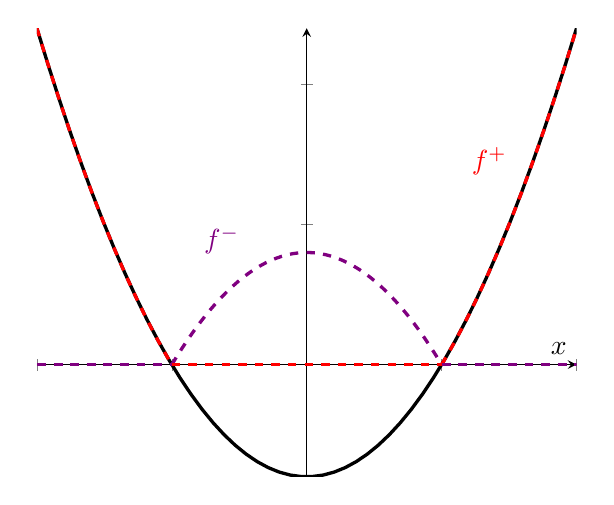
\begin{tikzpicture}
\begin{axis}[
axis y line=middle,
axis x line=middle,
xlabel=$x$,
%grid = both, %major/minor
xticklabels={},yticklabels={}
];

\addplot [
very thick,black,mark=none,
domain=-4:4,samples=50,
] {x^2 - 4)};

\addplot [
very thick,red,mark=none, dashed,
domain=-4:-2,samples=50,
] {x^2 - 4)};
\addplot [
very thick,red,mark=none, dashed,
domain=2:4,samples=50,
] {x^2 - 4)};
\addplot [
very thick,violet,mark=none,dashed,
domain=-2:2,samples=50,
] {abs(x^2 - 4))};

\addplot [
very thick,violet,mark=none,dashed,
domain=-4:-2,samples=50,
] {0};
\addplot [
very thick,violet,mark=none,dashed,
domain=2:4,samples=50,
] {0};

\addplot [
very thick,red,mark=none,dashed,
domain=-2:2,samples=50,
] {0};
\end{axis}
\node[color=red,right] at (5.4,4) {$f^+$};
\node[color=violet,right] at (2,3) {$f^-$};
\end{tikzpicture}$$

que verifican las siguientes propiedades:
\begin{enumerate}
\item $f^+ \; \land \; f^-$ son medibles y no negativas.
\item $f^+ - f^- = f$. 
\item $f^+ + f^- = \vert f \vert$
\item $f^+ \le \vert f \vert\; \land \;f^- \le \vert f \vert$ 
\end{enumerate}    
\end{defi}

\begin{prop}
Si $f: \mathbb{R}^n\rightarrow\mathbb{R}$ es una función integrable, entonces $f^+$ y $f^-$ son integrables, es decir:
\begin{align*}
\int_{\mathbb{R}^n} f^+ \dif{\mu} < +\infty & & \int_{\mathbb{R}^n} f^- d \mu < +\infty
\end{align*}
\end{prop}
\begin{demo}
Basta con ver que ambas funciones están acotadas por el módulo de $f$ y, por tanto, si $f$ es integrable, estas también lo son.
\end{demo}

En consecuencia, podemos dar una definición alternativa de la que se ha dado de función integrable que es completamente compatible e intercambiable con la que se ha dado anteriormente.

\begin{defi}
Sea $f: \mathbb{R}^{n} \rightarrow \mathbb{R}$ una función integrable, entonces podemos expresar su integral como: 
$$\int_{\mathbb{R}^n} f \dif{\mu} = \int_{\mathbb{R}^n} f^+ \dif{\mu} - \int_{\mathbb{R}^n} f^- \dif{\mu}$$
\end{defi}

\begin{obs}
Podríamos dar la misma definición de integrabilidad que se dió para funciones arbitrarias, pero ahora para funciones que toman valores en la recta ampliada. Sin embargo, cabe observar que $A=\{x\in \mathbb{R}: |f(x)|< \infty\}$ tiene que tener medida en caso de que dicha función sea integrable, puesto que:
$$\mu(A) > 0 \Rightarrow \forall k \in \mathbb{N}: k\cdot \chi_A \leq |f| \Rightarrow \int_{\mathbb{R}^n} |f| \ d\mu \geq I(k\chi_A) = k \cdot \mu(A)$$
\end{obs}

\begin{prop}
Supongamos que tenemos dos funciones $f,g: \mathbb{R}^n \rightarrow [-\infty, \infty]$ y tales que $f=g$ (c.t.p.), entonces tenemos que:
$$f \mbox{ integrable }\Leftrightarrow g \mbox{ integrable}$$
Y además las integrales coinciden:
$$\int_{\mathbb{R}^n} f \dif{\mu} = \int_{\mathbb{R}^n} g \dif{\mu}$$
\end{prop}
\begin{demo}
Como ya lo tenemos demostrado para funciones no negativas, basta con trabajar con las funciones $f^+$ y $f^-$, es decir:
$$f=g \ \mbox{c.t.p.}\Rightarrow \begin{cases}
f^+ = g^+ \\ f^- = g^- 
\end{cases} \mbox{c.t.p.}\Rightarrow \int f = \int f^+ - \int f^- = \int g^+ - \int g^- = \int g$$
\end{demo}

\begin{prop}
Son equivalentes:
\begin{itemize}
\item $f$ integrable
\item $|f|$ integrable
\item $f^+$ y $f^-$ integrables
\end{itemize}
\end{prop}
\begin{demo}
\begin{itemize}
\item $3)\rightarrow 1)$
$$\int |f| = \int f^+ + \int f^- < \infty \Rightarrow f \mbox{ integrable}$$
\end{itemize}
\end{demo}

\begin{lema}
Sea $f$ una función integrable, si $f = g - h$ con ambas funciones medibles, no negativas e integrables, entonces se verifica:
$$\int f \dif{\mu}= \int g \dif{\mu} - \int h \dif{\mu}$$
\end{lema}
\begin{demo}
Suponemos sin pérdida de generalidad que las funciones toman valores en $\bar{\mathbb{R}}$, puesto que más adelante se explica como generalizar dicho lema. De este modo, podemos expresar $f$ como:
$$f = f^+ - f^- = g-h\Rightarrow f^+ + h = f^- + g$$
Como todo son funciones no negativas e integrables, la integral de la suma es la suma de las integrales, por tanto:
$$\int f^+ + \int h = \int (f^+ + h) = \int (f^- + g)  = \int f^- + \int g \Rightarrow \int f^+ - \int f^- = \int g - \int h$$
\end{demo}

\begin{obs}
Este lema es válido para funciones que toman valores en $\bar{\mathbb{R}}$ porque el conjunto donde los valores no son reales es de medida nula. Por tanto, las funciones son iguales en c.t.p. a las funciones de la hipótesis y para esas la demostración es válida, luego para estas también.
\end{obs}

\begin{theo}[Operaciones de Integrabilidad]
Sean $f,g: \mathbb{R}^n \rightarrow \mathbb{R}$ dos funciones integrables, entonces la integral de la suma es:
$$\int (f+g) \dif{\mu} = \int f \dif{\mu} + \int g \dif{\mu}$$
Del mismo modo, para $\alpha \in \mathbb{R}$ la integral del producto por $\alpha$ es:
$$\int (\alpha \cdot f) \dif{\mu} = \alpha \int f \dif{\mu}$$
\end{theo}
\begin{demo}
Por la desigualdad triangular, $|f+g|\leq |f| + |g|$ y como ambas son funciones son no negativas, se les puede aplicar el lema:
$$\int |f+g| \leq \int |f| + \int |g| < \infty $$
De este modo, ya sabemos que al menos la suma es integrable, ahora veamos que la integral es justo la suma de las integrales. Para ello, expresamos la suma de la siguiente forma:
$$f+ g = f^+ - f^- + g^+ - g^- = (f^+ + g^+) - (f^- + g^-)$$
Como dichas funciones son  no negativas y son integrables, tenemos que
$$\int (f+g) = \int (f^+ + g^+) - \int (f^- + g^- ) = \int f^+ + \int g^+ - \int f^- +\int g^-  = \int f + \int g$$
Cabe observar que es necesario el lema para probar dicha demostración puesto que no se tiene en general la igualdad:
$$f^+ + g^+ = (f+g)^+$$
\end{demo}

\begin{theo}[De convergencia dominada]
Sea $\{f_k\}_{k=1}^{\infty}\rightarrow f$ una sucesión convergente c.t.p. a un a función $f$, donde las funciones $f_k: \mathbb{R}^n \rightarrow \mathbb{R}$ son medibles y $g: \mathbb{R}^n \rightarrow \left[0, +\infty\right]$ una función integrable que acota a $f$ c.t.p., es decir, $\vert f_k \vert \le g$ c.t.p., entonces:
$$\int_{\mathbb{R}^n} f \dif{\mu} = \lim_{k \rightarrow \infty} \int_{\mathbb{R}^n} f_k \dif{\mu}$$
\end{theo}
\begin{demo}
Sabemos que $\vert f \vert \le g$ c.t.p, luego tenemos que:
$$\int_{\mathbb{R}^n} \vert f \vert \dif{\mu} \le \int_{\mathbb{R}^n} g \dif{\mu} < +\infty$$
Por lo que ya sabemos que al menos $f$ es integrable (y por la misma razón las $f_k$ son integrables).

Como $\vert f_k \vert \le g \Rightarrow g + f_k \ge 0$, de este modo formamos la sucesión de funciones $\{g + f_k\}_{k=1}^{\infty}$ a la que podemos aplicar el lema de Fatou: 
$$\int_{\mathbb{R}^n} f \dif{\mu} + \int_{\mathbb{R}^n} g \dif{\mu} = \int_{\mathbb{R}^n} \left(f + g\right) \dif{\mu} = \int_{\mathbb{R}^n} \lim_{k \rightarrow \infty} \left(f_k + g\right) \dif{\mu} =\int_{\mathbb{R}^n} \liminf_{k \rightarrow \infty} \left(f_k + g\right)  \dif{\mu} \leq$$
$$ \stackrel{Fatou}{\le} \liminf_{k \rightarrow \infty}\int_{\mathbb{R}^n} \left(f_k + g\right) \dif{\mu} = \liminf_{k \rightarrow \infty} \left( \int_{\mathbb{R}^n} f_k \dif{\mu} + \int_{\mathbb{R}^n} g \dif{\mu} \right) = \left(\liminf_{k \rightarrow \infty} \int_{\mathbb{R}^n} f_k \dif{\mu}  \right) + \int_{\mathbb{R}^n} g \dif{\mu}$$
Luego ya tenemos la desigualdad
$$\int_{\mathbb{R}^n} f \dif{\mu} \le \liminf_{k \rightarrow \infty}\left( \int_{\mathbb{R}^n} f_k \dif{\mu}\right)$$
De forma análoga, tomamos la sucesión $\{-f_k + g\}_{k=1}^{\infty}$ y entonces:
$$\int_{\mathbb{R}^n} \left(-f\right) \dif{\mu} \le \liminf_{k \rightarrow \infty} \int_{\mathbb{R}^n} \left(-f_k\right) \dif{\mu} \Rightarrow - \int_{\mathbb{R}^n} f \dif{\mu} \le \liminf_{k \rightarrow \infty} \left(-\int_{\mathbb{R}^n} f_k \dif{\mu} \right) =$$
$$= -\limsup_{k \rightarrow \infty} \left(\int_{\mathbb{R}^n} f_k \dif{\mu} \right) \Rightarrow \Rightarrow \limsup_{k \rightarrow \infty} \int_{\mathbb{R}^n} f_k \dif{\mu} \le \int_{\mathbb{R}^n} f \dif{\mu} $$
Como por la convergencia, se tiene que el límite superior e inferior coinciden con el límite global, se tiene la igualdad.
\end{demo}

\subsection{Cálculo de integrales en \texorpdfstring{$\mathbb{R}^n$}{Rn}}
A pesar de que hemos definido todos los conceptos relativos al cálculo de integrales en $\mathbb{R}^n$, hasta ahora no hemos visto ningún método efectivo en términos prácticos para calcular integrales superiores a una dimensión. Aquí se desarrolla el Teorema fundamental que nos permite simplificar el cálculo de integrales en $\mathbb{R}^n$ al cálculo de varias integrales en $\mathbb{R}$.

\begin{defi}[Secciones de funciones]
Sea $f: \mathbb{R}^{n} \times \mathbb{R}^n \rightarrow \mathbb{R}$ una función que expresaremos como $f \left(x, y\right)$ donde $x \in \mathbb{R}^n$ y $y \in \mathbb{R}^n$, llamamos \textbf{secciones} de $f$ a:
$$\forall x \in \mathbb{R}^n, \ f_x: \mathbb{R}^n \rightarrow \mathbb{R} \mbox{ donde } f_x \left(y\right) = f \left(x, y\right)$$
\end{defi}

\begin{lema}
Si $f$ y $g$ verifican el Tª de Tonelli y $a, b \in \mathbb{R}^+$, entonces la composición lineal de las funciones también, es decir, $af + bg$ cumple el Tª de Tonelli.
\end{lema}
\begin{demo}
Se ha de demostrar que en primer lugar, se tiene que:
$$\left(af + bg\right)_x = af_x + bg_x$$
Esta combinación lineal será medible, por serlo de funciones medibles y, por tanto:
$$F_{af + bg} = aF_f + bF_g$$ 
\end{demo}

\begin{lema}
Si una sucesión de funciones $\{f_k\}_{k=1}^{\infty}$ convergente puntualmente a $f$ cumple el Tª de Tonelli, entonces $f$ cumple el Tª Tonelli. 
\end{lema}
\begin{demo}
\begin{enumerate}
    \item Primero, vemos que
    $$f_x = \lim_{k \rightarrow \infty} \left(f_k\right)_x,\ \left(f_k\right)_x \uparrow f_x $$
    que es medible por ser límite de medibles
    \item En segundo lugar, como: 
    $$F = \lim_{k \rightarrow \infty}F_k,\ \{F_k\}_{k=1}^{\infty} \uparrow F \Rightarrow\lim_{k \rightarrow \infty} \int_{\mathbb{R}^m} \left(f_k\right)_x \dif{\mu} = \int_{\mathbb{R}^m} f_x \dif{\mu} $$
    \item Por último, tenemos que: 
    $$\int_{\mathbb{R}^n} F \dif{\mu} = \int_{\mathbb{R}^n} \lim_{k \rightarrow \infty}F_k  \dif{\mu} = \lim_{k \rightarrow \infty}\int_{\mathbb{R}^n} F_k \dif{\mu} = \lim_{k \rightarrow \infty} \int_{\mathbb{R}^n \times \mathbb{R}^m} f_k  \dif{\mu} = \int_{\mathbb{R}^n} f \dif{\mu}  $$
\end{enumerate}
\end{demo}

Como consecuencia de estos lemas el principio de Cavalieri es equivalente al teorema de Tonelli, es decir, basta con probar este principio para probar el teorema de Tonelli.

\begin{theo}[de Tonelli]
Sea $f: \mathbb{R}^{n} \times \mathbb{R}^m \rightarrow \left[0, +\infty\right)$ una función medible, entonces: 
\begin{enumerate}
    \item Para casi todo $x \in \mathbb{R}^n$, $f_x$ es medible en $\mathbb{R}^n$ (y no negativa).
    \item La función $F: \mathbb{R}^{n} \rightarrow \left[0, +\infty\right]$ es medible, donde se define como:
        $$F \left(x\right) = \int_{\mathbb{R}^m} f_x \dif{\mu_m} $$
    \item Se puede dividir la integral en secciones, es decir:
        $$\int_{\mathbb{R}^n \times \mathbb{R}^m} f \ \dif{\mu_{nm}} = \int_{\mathbb{R}^n} F \dif{\mu_n} $$
    expresado de forma más intuitiva:
    $$\int_{\mathbb{R}^n \times \mathbb{R}^m} f \left(x, y\right) \dif{x}\dif{y} = \int_{\mathbb{R}^n}\left(\int_{\mathbb{R}^m} f \left(x, y\right) \dif{y} \right)\dif{x} = \int_{\mathbb{R}^m}\left(\int_{\mathbb{R}^n} f \left(x, y\right) \dif{x} \right)\dif{y}$$
\end{enumerate}
Este teorema se podría enunciar de forma análoga para $y$, siendo entonces las hipótesis:
\begin{enumerate}
\item Para casi todo $y \in \mathbb{R}^m$, $f_y$ es medible en $\mathbb{R}^m$ (y no negativa).
\item La función $G: \mathbb{R}^n \rightarrow \left[0, \infty\right]$ es medible, donde se define como:
$$G \left(x\right) = \int_{\mathbb{R}^n} f_x \dif{\mu}$$
\item Se puede dividir la integral en secciones, es decir:
$$\int_{\mathbb{R}^n \times \mathbb{R}^m} f \dif{\mu} = \int_{\mathbb{R}^n} G \dif{\mu},$$
expresado de forma más intuitiva:
$$\int_{\mathbb{R}^n \times \mathbb{R}^m} f \left(x, y\right) \dif{x}\dif{y} = \int_{\mathbb{R}^m} \left(\int_{\mathbb{R}^n} f \left(x, y\right) \dif{x} \right) \dif{y}.$$
\end{enumerate}
\end{theo}
\begin{demo}
Para demostrar este teorema para funciones no negativas se irá demostrando para funciones más sencillas e incrementaremos la complejidad de forma gradual hasta llegar a las de las hipótesis.

\begin{enumerate}
\item Primeramente consideramos $f = \chi_{Q}$ donde $Q \subset \mathbb{R}^{n+m}$ es un cubo semiabierto, es decir, $Q = \prod_{i=1}^{n+m} \left[a_i, b_i\right)$. Este cubo se puede expresar en términos de otros dos, esto es, $Q = A \times B$ con $A \subset \mathbb{R}^n$ y $B \in \mathbb{R}^m$ cubos semiabiertos. Veamos entonces que:
\begin{enumerate}
    \item
    $$\left(\chi_Q\right)_x = \chi_{Q_x} = \begin{cases} \chi_B &  x \in A\\ 0 &  x \not\in A \end{cases} \Rightarrow \left(\chi_Q\right)_x$$
    $$\text{ ya que }Q_x = \begin{cases} B & x\in A \\ \emptyset & x\notin A \end{cases}\Rightarrow \chi_{Q_x} \text{ medible }\forall x \in \mathbb{R}^n$$
    \item
    $$F \left(x\right) = \int_{\mathbb{R}^m} \chi_{Q_x} \dif{\mu_m} = \begin{cases} \int_{\mathbb{R}^m} \chi_b \dif{\mu_m} = \mu_m \left(B\right) & x \in A \\ 0 & x \not\in A\end{cases} \text{ medible} \Rightarrow$$
    $$F \left(x\right) = \mu_m \left(B\right)\cdot \chi_A \left(x\right)$$
    \item
    $$\int_{\mathbb{R}^n} F \left(x\right) \dif{\mu_n} = \mu_m \left(B\right) \cdot \mu_n \left(A\right) = \mu_{n+m} \left(Q\right) = \int_{\mathbb{R}^n \times \mathbb{R}^m} \chi_Q \dif{\mu_{m+n}} $$
    Siendo la 2 igualdad cierta por tratarse de un cubo.
\end{enumerate}
\item Consideramos ahora $f = \chi_G$ donde $G \subset \mathbb{R}^{n+m}$ es un abierto. Por serlo, podemos escribirlo como $G = \bigsqcup_{j=1}^{\infty} Q_j$ donde cada $Q_j$ es un cubo semiabierto y la unión es disjunta.

Denotando $G_k = \bigsqcup_{j=1}^{k} Q_j$ tenemos que $\chi_{G_k} = \sum_{j=1}^{k} \chi_{Q_j}$. Por ser dicha función característica suma finita de funciones características de cubos (que ya sabemos que cumplen el Teorema), también cumple el Teorema por el primer lema y además vemos que $\{\chi_{Q_k}\}_{k=1}^{\infty} \uparrow \chi_G$ puntualmente, luego:
$$\chi_G = \sum_{j=1}^{\infty} \chi_{G_j} = \lim_{k \rightarrow \infty}\chi_{G_k} $$
De este modo, basta con aplicar el segundo lema y cumple el Teorema.

\item Supongamos que $f = \chi_D$ donde $D \subset \mathbb{R}^{n + m}$ es un conjunto $G_\delta$. En este caso, es suficiente considerar que $D$ es acotado puesto que $D$ se puede expresar como una unión creciente $$D = \bigcup_{k=1}^{\infty} D_k$$ donde cada $D_k$ es un $G_\delta$ y acotado (por ejemplo, $D_k = D \cap \left(-k, k\right)^{n+m}$). De este modo, $\{\chi_{D_k}\}_{k=1}^{\infty} \uparrow \chi_D$ y usando el segundo lema, ya lo tendríamos.

En consecuencia, supongamos que $D$ es $G_\delta $ y acotado, entonces escribimos
$$D = \bigcap_{k = 1}^{\infty} G_k$$
donde cada $G_k$ es abierto acotado y $G_1 \supset G_2 \supset G_k \supset \ldots \supset D$. De este modo, construimos la sucesión $\{\chi_{G_k}\}_{k=1}^{\infty} \downarrow \chi_D$ con la que, usando la versión decreciente de TCM, se puede hacer una demostración análoga a la del segundo lema para obtener que $\chi_D$ verifica el teorema. 

Alternativamente, como $0 \le \chi_D \le \chi_{G_1}$ es integrable y satisface el teorema, entonces se puede aplicar el TCD.

\item Consideramos ahora $f = \chi_N$ donde $\mu_{n+m} \left(N\right) = 0$. Por la regularidad de la medida, tenemos que:
$$\forall k \in \mathbb{N},\ \exists G_k \subset \mathbb{R}^{n+m} \mbox{ abierto con } N \subset G_k  \mbox{ y }  \mu_{n+m} \left(G_k \setminus N\right) < \frac{1}{k}$$

Si definimos $G:= \bigcap_{k \in \mathbb{N}} G_k$, entonces vemos que $G$ es un $G_\delta$ por ser intersección numerable de abiertos, tal que $N \subset G $ y además: 
$$\mu_{n+m} \left(G\setminus N\right) \le \forall k \in \mathbb{N}: \mu_{n+m} \left(G_k \setminus N\right) < \frac{1}{k} \xrightarrow{k\rightarrow \infty} 0 \Rightarrow \mu_{n+m}(G) = 0$$

De este modo, hemos encontrado un $G_\delta$ que contiene a $N$. En primer lugar, vemos que $\chi_G$ satisface el teorema para casi todo $x \in \mathbb{R}^n$ por el apartado anterior y, por tanto, $\chi_G$ es medible, luego:
$$0 = \mu_{n+m} \left(G\right) = \int_{\mathbb{R}^n \times \mathbb{R}^m} \chi_{G} \dif{\mu_{n+m}} = \int_{\mathbb{R}^n} \left( \int_{\mathbb{R}^m} \chi_{G_x}  \dif{\mu_m} \right) \dif{\mu_n}.$$
Por tanto, como la integral de dentro es la $F(x)$ del enunciado y es positiva:
$$\mu_m \left(G_k\right) = \int_{\mathbb{R}^m} \chi_{G_x} \dif{\mu_m} = 0 \text{ en casi todo punto } x \in \mathbb{R}^n$$
Como $N_x \subset G_x\Rightarrow \mu_m(N_x) \leq \mu_m(G_x) = 0 \Rightarrow \mu_m(N_x) = 0$ y además es medible, luego tenemos que $\chi_{N_x} = \left(\chi_N\right)_x = f_x$ es medible en para c.t.p. de $\mathbb{R}^n$.

Para la segunda consecuencia basta ver que:
$$0 \le F \left(x\right) = \int_{\mathbb{R}^m} \chi_{N_x} \dif{\mu_m} \le \int_{\mathbb{R}^m} \chi_{G_x} \dif{\mu_m} = 0 \text{ c.t.p. } \in \mathbb{R}^n$$
Por lo que, en particular, $F$ es medible.

Y, por último, hay que ver que la integral se puede iterar:
$$\int_{\mathbb{R}^n \times \mathbb{R}^m} \chi_N \dif{\mu_{n+m}} = 0 = \int_{\mathbb{R}^n} \underbrace{F \left(x\right)}_{=0} \dif{\mu_n} = \int_{\mathbb{R}^n} \left(\int_{\mathbb{R}^m} \chi_{N_x} \dif{\mu_m} \right) \dif{\mu_n} $$

\item Sea ahora $f = \chi_A$ donde $A \subset \mathbb{R}^{n+m}$ es medible. Por ser medible, sabemos que podemos descomponer $A$ como $A = D \setminus N$, donde $D$ es un $G_\delta $ y $\mu_{n+m} \left(N\right) = 0$. Por tanto, $D = A \sqcup N \Rightarrow \chi_D = \chi_A + \chi_N$ y, en consecuencia:
$$\chi_A = \chi_D - \chi_N \text{ para c.t.p. } x \in \mathbb{R}^n$$
Y es sencillo ver que también se cumple la igualdad:
$$\chi_{A_x}= \chi_{B_x} - \chi_{N_x} \text{ es medible por (3) y (4)}$$

Para ver la segunda conclusión, tenemos que: 
$$F \left(x\right) = \int_{\mathbb{R}^m} \chi_{A_x} \dif{\mu_m} = \int_{\mathbb{R}^m} \chi_{D_x} \dif{\mu_m}$$
puesto que $\mu_m \left(N_x\right) = 0$ y entonces es medible para c.t.p. $x \in \mathbb{R}^n$ porque $D$ es $G_\delta$ y aplicamos el apartado (3).

Para terminar:
$$\int_{\mathbb{R}^n} F \left(x\right) \dif{\mu_n} = \int_{\mathbb{R}^n} \left( \int_{\mathbb{R}^m} \chi_{A_x} \dif{\mu_m} \right) \dif{\mu_n} = \int_{\mathbb{R}^n} \left(\int_{\mathbb{R}^m} \chi_{D_x} \dif{\mu_m} \right) \dif{\mu_n} = $$
$$= \int_{\mathbb{R}^n \times \mathbb{R}^m} \chi_{D} \dif{\mu_{n+m}} = \mu_{n+m} \left(D\right) = \mu_{n+m} \left(A\right) = \int_{\mathbb{R}^n \times \mathbb{R}^m} \chi_A \dif{\mu_{n+m}} $$
Porque $D_x$ si verificaba ya el Teorema de Tonelli.

\item Sea $f$ función simple, medible, no negativa, entonces $f$ es combinación lineal no negativa de funciones características de conjuntos medibles en $\mathbb{R}^n \times \mathbb{R}^m$ y por el lema trivialmente se tiene.

\item Finalmente, consideramos $f$ medible no negativa. Como para estas funciones hemos demostrado que $ \exists \{f_k\}_{k=1}^{\infty}\uparrow f$ donde cada $f_k$ es simple, medible y no negativa, queda probado por el lema 2 y el apartado 6.
\end{enumerate} 
\end{demo}

\begin{defi}[Secciones de conjuntos]
Si tenemos un conjunto $A \subset \mathbb{R}^n \times \mathbb{R}^m$, podemos definir su \textbf{sección} como:
$$A_x = \{y \in \mathbb{R}^m: \left(x, y\right) \in A\}$$
\end{defi}
\begin{prop}[Principio de Cavalieri]
Sea $A \subset \mathbb{R}^n \times \mathbb{R}^m$ medible, entonces: 
\begin{enumerate}
    \item Los $A_x$ son medibles c.t.p $x\in \mathbb{R}^n$.
    \item La función $F: \mathbb{R}^n \rightarrow \left[0, +\infty\right]$ es medible y se define como:
    $$F \left(x\right) = \mu_m \left(A_x\right)$$
    \item $\mu_{n+m} \left(A\right) = \int_{\mathbb{R}^n} \mu_m \left(A_x\right) \dif{\mu_n} $
\end{enumerate}
\end{prop}

$$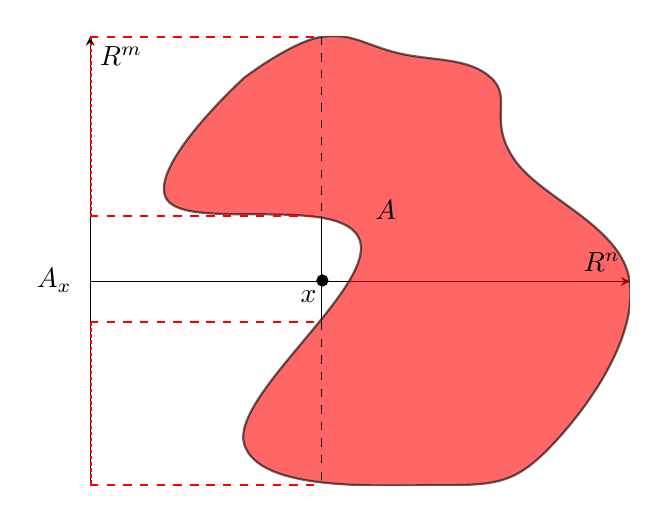
\begin{tikzpicture}
\begin{axis}[
tick style={draw=none},
axis y line=middle,
axis x line=middle,
xlabel=$\mathbb{R}^n$,
ylabel=$\mathbb{R}^m$,
xticklabels={},yticklabels={}
%grid = both, %major/minor
];
\addplot [thick, domain=0:7,fill=red, opacity=0.6]  plot[smooth, tension=.7] coordinates {(2,2.5) (3,3) (4,2.8) (5.2,2.5) (5.5,1.5) (7,0) (6,-2)(4.5,-2.5) (2,-2) (3.5,0.5) (1,1) (2,2.5)};

\draw [dashed] (3,3) -- (3,0.8);
\draw [solid] (3,0.8) -- (3,-0.5);
\draw [dashed] (3,-0.5) -- (3,-3);

\draw [densely dotted, very thick, red] (0,3) -- (0,0.8);
\draw [densely dotted, very thick, red] (0,-0.5) -- (0,-2.5);

\addplot [domain=0:3, samples=100, thick, color=red, dashed]{3};
\addplot [domain=0:3, samples=100, thick, color=red, dashed]{0.8};
\addplot [domain=0:3, samples=100, thick, color=red, dashed]{-0.5};
\addplot [domain=0:3, samples=100, thick, color=red, dashed]{-2.5};       
   

\end{axis}
\filldraw [black] (2.95,2.6) circle (2pt);
\node[color=black,right] at (-0.8,2.6) {$A_x$};
\node[color=black,right] at (2.55,2.4)  {$x$};
\node[color=black,right] at (3.5,3.5) {$A$};
\end{tikzpicture}$$

\begin{obs}
Si $N \subset \mathbb{R}^{n+m}$ satisface que $\mu_{n+m} \left(N \right) = 0$ hemos visto que para casi todo $x \in \mathbb{R}$ la sección $N_x$ es medible porque tiene medida nula. Sin embargo, puede ocurrir que para algún $x \in \mathbb{R}^n$ la sección $N_x$ no sea medible en $\mathbb{R}^m$

Por ejemplo, sea $E \subset \mathbb{R}$ no medible y sea $N = \{0\} \times E \subset \mathbb{R}^2$. Como $N$ está contenido en la recta $\{0\} \times \mathbb{R}$ está claro que $\mu_2 \left(N\right) = 0$, pero la sección $N_0 = E$ no es medible.
\end{obs}

\begin{coro}
Si la medida del conjunto es nula, entonces la medida de casi todas las secciones también lo es.
$$\mu_{n + m} \left(A\right) = 0 \Rightarrow \mu_m \left(A_x\right) = 0 \text{ c.t.p } x$$
\end{coro}

\begin{ej} 
Si $A \subset \mathbb{R}^n \times \mathbb{R}^m$:
$$\int_A f \left(x, y\right) \dif{x} \dif{y} = \int_{\mathbb{R}^n \times \mathbb{R}^m} f \left(x, y\right) \chi_A \left(x, y\right) \dif{x}\dif{y} = $$
$$\int_{\mathbb{R}^n} \left(\int_{\mathbb{R}^m} f \left(x, y\right) \chi_A \left(y\right) \dif{y} \right) \dif{x} = \int_{\mathbb{R}^n} \left(\int_{A_x} f \left(x, y\right) \dif{y}\right) \dif{x}$$
\end{ej}

\begin{theo}[de Fubini]
Sea $f: \mathbb{R}^n \times \mathbb{R}^m \rightarrow \mathbb{R}$ integrable. Entonces: 
\begin{enumerate}
\item Para c.t.p. $x \in \mathbb{R}^n$, $f_x$ es medible en $\mathbb{R}^n$ (y no negativa).
\item La función $F: \mathbb{R}^n \rightarrow \left[0, \infty\right]$ es medible en $\mathbb{R}^n$, donde $F$ está definida en c.t.p. como:
$$F \left(x\right) = \int_{\mathbb{R}^m} f_x \dif{\mu}_m$$

\item Se puede dividir la integral en secciones, es decir:
$$\int_{\mathbb{R}^n \times \mathbb{R}^m} f \dif{\mu}_{n+m} = \int_{\mathbb{R}^n} F \dif{\mu}_n,$$
\end{enumerate}
\end{theo}
\begin{demo}
\begin{enumerate}
Podemos escribir $f = f^+ - f^-$. De nuevo, es sencillo ver que $\forall x \in \mathbb{R}^n : \left(f^+\right)_x = \left(f_x\right)^+ \; \land \; \left(f^-\right)_x = \left(f_x\right)^-$, por tanto como $f^+$ y $f^-$ verifican el teorema de Tonelli, entonces $f^+_x $ y $f^-_x$ son medibles c.t.p $x \in \mathbb{R}^n$ y como $f_x = \left(f^+_x\right) - \left(f^-_x\right)$ también es medible c.t.p $x \in \mathbb{R}^n$.

Tanto la $f^+$ como la $f^-$ son integrales porque:
 $$\int_{\mathbb{R}^n} \left(\int_{\mathbb{R}^m} f^+_x \dif{\mu_m} \right) \dif{\mu_n} = \int_{\mathbb{R}^n \times \mathbb{R}^m} f^+ \dif{\mu_{n+m}} < \infty$$
Por tanto, $F \left(x\right) = \int_{\mathbb{R}^n} f^+_x \dif{\mu_n} + \int_{\mathbb{R}^n} f^-_x \dif{\mu_n}$ es finita en c.t.p., luego integrable.
\end{enumerate}
\end{demo}

\begin{obs}
El problema, en general, es demostrar que una función es integrable para poder aplicar este teorema. Un método útil suele ser demostrar que $\int_{\mathbb{R}^n} \left(\int_{\mathbb{R}^m} \vert f \left(x, y\right) \vert \dif{y} \right) \dif{x} < \infty$ y como con el valor absoluto es no negativa podemos aplicar Tonelli a $\vert f\vert$ y separar la integral para demostrar que $f$ es integrable.
\end{obs}

\begin{ej}
Consideramos $E = \{ \left(x, y\right) \in \mathbb{R}^2 : 0 \leq x \leq y\}$ y $f \left(x, y\right) = e^{-y^2}$ y vamos a ver que es integrable en $E$ y a calcular su integral:
\begin{itemize}
    \item En primer lugar, $f \left(x, y\right) = e^{-y^2} \ge 0$ es medible por ser continua en $\mathbb{R}^2$.
    \item En segundo lugar, como es positiva por el Teorema de Tonelli es integrable y la integral se puede calcular como: 
    $$\int_E f \left(x, y\right) \dif{x} \dif{y} = \int_{\mathbb{R}^2} f \left(x, y\right) \cdot \chi_{E} \left(x, y\right) \dif{x} \dif{y} = \int_{-\infty}^{\infty} \int_{-\infty}^{\infty} e^{-y^2}\chi_E \left(x, y\right) \dif{x} \dif{y} =$$
    $$=\int_{0}^{\infty} \int_{0}^{y} e^{-y^2} \dif{x} \dif{y} = \frac{1}{2} \int_{0}^{\infty} 2ye^{-y^2} \dif{y} = \left[\frac{1}{2} \left(e^{-y^2}\right)\right]_{y=0}^{y=\infty} = \frac{1}{2} \left(1 - 0\right) =\frac{1}{2}$$
\end{itemize}
\end{ej}

\begin{prop}
Sea $f: \left[a, \infty\right) \rightarrow \left[0, +\infty\right)$ continua, entonces la integral impropia coincide con la impropia de Riemann
$$\int_{[a, +\infty)} f = \lim_{R \rightarrow \infty} \int_a^R f $$
Nótese que esto se refiere a funciones \textbf{positivas}.
\end{prop}
\begin{demo}
Sea $a \le \{b_k\}{k=1}^{\infty}\uparrow \infty$ y definimos $f_k = f \cdot \chi{\left[a, b_k\right]}$. Así, $\{f_k\}_{k=1}^{\infty}\uparrow f$ luego por el Teorema de la Convergencia Monótona
$$\int_{\left[a, \infty\right)} f = \lim_{k \rightarrow \infty} \int_{\left[a, \infty\right)} f_k = \lim_{k \rightarrow \infty} \int_a^{b_k} f $$
\end{demo}

\begin{ej}
Consideramos $A = \left[0, 1\right] \times \left[0, +\infty\right]$ y la función $f \left(x, y\right) = e^{-y} \sen \left(2xy\right)$ y vamos a demostrar que es integrable y a calcular la integral.
\end{ej}

\begin{itemize}
    \item En primer lugar, para poder aplicar el Teorema de Fubini, necesitamos ver que $f$ es integrable, es decir, $\int_A \vert f\vert < \infty$, luego calculamos:
    $$\vert f \left(x, y\right)\vert = \vert e^{-y} \sen \left(2xy\right)\vert \le e^{-y}$$
    $$\int_A \vert f \left(x, y\right) \vert \le \int_A e^{-y} \dif{x} \dif{y} = \int_0^1 \int_0^{\infty} e^{-y} \dif{y} \dif{x} = \left(\int_0^1 1 \dif{x}  \right) \left(\int_0^{\infty} e^{-y} \dif{y} \right) = 1 < \infty $$
\item Una vez que sabemos que es integrable, aplicamos Fubinni:
    $$\int_A f \left(x, y\right) \dif{x} \dif{y} = \int_0^1 \left(\underbrace{\int_0^{\infty} e^{-y}\sen\left(2xy\right) \dif{y}}_{F \left(x\right)} \right) \dif{x}  = **$$
    \begin{itemize}
    	\item Veamos primero la $F \left(x\right)$:
    $$\begin{cases}
        u = \sen \left(2xy\right) & du = 2x \cos \left(2xy\right)dy \\\\
        dv = e^{-y}dx & v = -e^{-y}
    \end{cases} \Rightarrow$$
    $$F \left(x\right) = \underbrace{\left[-e^{-y} \sen \left(x, y\right)\right]_{0}^{\infty}}_{= 0} + \int_0^{\infty} 2xe^{-y}\cos \left(2xy\right) \dif{y}$$
    $$\begin{cases}
        u = 2x\cos \left(2xy\right) & du = \left(2x\right)^2 \cdot \left(-\sen \left(2xy\right)\right)dy \\
        dv = e^{-y}dy & v = -e^{-y}
    \end{cases}$$
    $$F(x)=\left[-e^{-y}2x \cos \left(2xy\right)\right]_{0}^{\infty} - \int_0^{\infty} 4x^2e^{-y}\sen \left(2xy\right) \dif{y} = 2x - 4x^2 F \left(x\right)\Rightarrow$$
    $$\Rightarrow F \left(x\right) \cdot \left(1 + 4x^2\right) = 2x \Rightarrow F \left(x\right) = \frac{2x}{1+4x^2}$$
    	\item Volviendo a la integral original:
    $$\int_0^1 \frac{1}{4} \cdot \frac{8x}{1+4x^2} \dif{x} = \frac{1}{4} \left[\log \left(1 + 4x^2\right)\right]_{0}^{1} = \frac{\log \left(5\right)}{4}.$$
    \end{itemize}
\end{itemize}

\begin{prop}
Sea $f: \left[a, \infty\right) \rightarrow \mathbb{R}$ continua, si es integrable, entonces la integral impropia coincide con la impropia de Riemann:
$$\lim_{R \rightarrow \infty} \int_a^k f = \int_{\left[a, \infty\right)} f $$
Nótese que esto es cierto para funciones \textbf{con valores en $\mathbb{R}$}.
\end{prop}

\begin{demo}
Sea $a \le \{b_k\}{k=1}^{\infty}\uparrow \infty$ y sean $f_k = f \cdot \chi{\left[a, \infty\right)}$. Entonces, $ \{f_k\}k \rightarrow f$ puntualmente y además $\vert f_k \vert \le \vert f \vert \text{ ,que es integrable en } \left[a, \infty\right)$ Así, por el Teorema de la Convergencia Dominada, $$\lim{k \rightarrow \infty} \int_a^{b_k} f = \int_a^{\infty} f$$ 
\end{demo}

\begin{defi}[Funciones definidas por integrales]
Una función viene definida por una integral si tiene la siguiente forma: 
$$F \left(u\right) = \int_{\mathbb{R}^n} f \left(x, u\right) \dif{x} $$
Donde para un $u$ fijo, se integra la función sobre las componente $x$ libre y en su medida concreta.
\end{defi}

\begin{theo}
Sea $\mathcal{U} \subset \mathbb{R}^m$ y sea $f: \mathbb{R}^n \times \mathcal{U} \rightarrow \mathbb{R}$, supongamos que: 
\begin{enumerate}
    \item $\forall u \in \mathcal{U},\ f_{u}: \mathbb{R}^n \rightarrow \mathbb{R}$ es integrable.
    \item $\forall x \in \mathbb{R}^n,\ f_x: \mathcal{U} \rightarrow \mathbb{R}$ es continua.
    \item $\exists g: \mathbb{R}^n \rightarrow \mathbb{R}$ integrable tal que $\vert f \left(x, u\right) \vert \le g \left(x\right),\ \forall x \in \mathbb{R}^n,\ \forall u \in \mathcal{U}$
\end{enumerate}
Entonces se verifica la continuidad de la definida por la integral: 
$$F \left(u\right) = \int_{\mathbb{R}^n} f \left(x, u\right) \dif{x} \text{ es continua en } \mathcal{U}.$$
\end{theo}
\begin{demo}
Sea $\{u_k\}_{k=1}^{\infty} \subset \mathcal{U}$ con $u_k \rightarrow u_0$ en $\mathcal{U}$, definimos $\forall k \in \mathbb{N}: f_k = f{u_k} = f \left(x, u_k\right) \rightarrow f \left(x, u\right)$. Además, como se tiene que $\vert f_k \left(x\right) \vert = \vert f \left(x, u_k\right) \vert \le g \left(x\right)$ y esto para $\forall x \in \mathbb{R}^n$ y $\forall k \in \mathbb{N}$, por el TCM: 
$$\underbrace{\int_{\mathbb{R}^n} f_k \left(x\right) \dif{x}}_{F \left(u_k\right)} \rightarrow \underbrace{\int_{\mathbb{R}^n} f \left(x, u_0\right) \dif{x}}_{= F \left(u_0\right)} $$
\end{demo}

\begin{theo}[Regla de Leibniz]
Sea $f: \mathbb{R}^{n} \times \left[a, b\right] \rightarrow \mathbb{R}$ una función medible y $F \left(t\right) = \int_{\mathbb{R}^n} f \left(x, t\right) \dif{x}$ la definida por la integral de dicha función, supongamos que: 
\begin{enumerate}
    \item $\forall r \in \left[a, b\right],\ f_r: \mathbb{R}^{n} \rightarrow \mathbb{R}$ es integrable en $\mathbb{R}^n$.
    \item $\forall x \in \mathbb{R}^n : \ f_x: \left[a, b\right] \rightarrow \mathbb{R}$ es $C^{1)}$, donde $f_x \left(t\right) = f \left(x, t\right)$
    \item $\exists g: \mathbb{R}^n \rightarrow \mathbb{R}$ integrable tal que $\vert \frac{\partial f \left(x, t\right)}{\partial t}\vert \le g \left(x\right) : \forall x \in \mathbb{R}^n \mbox{ y }\forall k \in \left[a, b\right]$
\end{enumerate}
Entonces $F$ es $C^{1)}$ en $\left(a, b\right)$ y $\forall t \in \left(a, b\right)$ podemos definir su derivada: 
$$F' \left(t\right) = \int_{\mathbb{R}^n} \frac{\partial f \left(x, t\right)}{\partial t} \dif{x} $$
\end{theo}
\begin{demo}
Vamos a aplicar el Teorema de Fubini y de Tonelli a $\frac{\partial f\left(x, t\right)}{\partial t} $
\begin{itemize}
    \item En primer lugar, como podemos expresar dicha función como: 
    $$\frac{\partial f}{\partial t} \left(x, t\right) = \lim_{s \rightarrow 0^+} \frac{f \left(x, t + s\right) - f \left(x, t\right)}{s} = \lim_{k \rightarrow \infty} \frac{f \left(x, t + \frac{1}{k}\right) - f \left(x, t\right)}{\frac{1}{k}}$$
    es medible por ser límite puntual de funciones medibles.
    \item En segundo lugar, como podemos acotarla por una función integrable, es integrable en $\mathbb{R}^n \times \left[a, b\right]$:
    $$\int_{\mathbb{R}^n} \left\vert \frac{\partial f}{\partial t} \left(x, t\right)\right\vert  \dif{x} \dif{y} \le \int_{\mathbb{R}^n \times \left[a, b\right]} g \left(x\right) \dif{x} \dif{t} = \int_{\mathbb{R}^n} \left(\int_a^b g \left(x\right) \dif{t}  \right) \dif{x}  = $$
    $$ = \int_{\mathbb{R}^n} \left(b - a\right) g \left(x\right) \dif{x} = \left(b - a\right) \int_{\mathbb{R}^n} g(x) \dif{x}< +\infty$$
    \item Aplicamos el teorema de Fubini, es decir, $\forall s \in \left[a, b\right]$: 
    $$\int_a^s \left(\int_{\mathbb{R}^n} \frac{\partial f}{\partial t} \left(x, t\right) \dif{x} \right) \dif{t} = \int_{\mathbb{R}^n} \left(\int_a^s \frac{\partial f}{\partial t} \left(x, t\right) \dif{t} \right) \dif{x} = $$
    $$= \int_{\mathbb{R}^n} \left( f \left(x, s\right) - f \left(x, a\right)\right) \dif{x} = F \left(s\right) - F \left(a\right).$$
    Denotamos: 
    $$H \left(t\right) := \int_{\mathbb{R}^n} \frac{\partial f\left(x, t\right)}{\partial t}  \dif{x}$$
    Como $\frac{\partial f\left(x, t\right)}{\partial t}  = f_x' \left(t\right)$ es continua en $t$ y $\vert \frac{\partial f}{\partial t} \vert \le g$, por el Teorema anterior obtenemos que $H$ es continua en $t \in \left[a, b\right]$. En consecuencia, vemos que: 
    $$\int_a^s H \left(t\right) \dif{t} = F \left(s\right) - F \left(a\right) \Rightarrow F \left(s\right) = F \left(a\right) + \int_a^s H \left(t\right) \dif{t}$$
	Por el Teorema Fundamental del Cálculo:    
    $$F' \left(t\right) = H \left(t\right),\ \forall t \in \left(a, b\right) $$
\end{itemize}
\end{demo}

\begin{ej}
Supongamos la función 
$$F \left(t\right) = \int_0^{\infty} \frac{1 - e^{tx}}{xe^{x}} \dif{x} \text{\quad con } t > -1$$
En primer lugar, veamos que $F$ está bien definida y que es derivable en $t \in \left(-1, \infty\right)$:

Dado $t \in \left(-1, \infty\right)$ sean $-1 < a < t_0 < b <\infty$. Vamos a demostrar que $F$ es derivable $\left(C^1\right)$ en $\left(a, b\right)$. De aquí se deduce que $F$ es derivable $\left(C^1\right)$ en $\left(-1, \infty\right)$.

\begin{enumerate}
    \item En primer lugar, veamos que $\forall t > -1: f_t \left(x\right) = \frac{1 - e^{-tx}}{x} e^{-x}$ es una función integrable en $\left(0, \infty\right)$:
    $$\lim_{x \rightarrow 0^+} \frac{1 - e^{-tx}}{x} = \lim_{x \rightarrow 0^+} \frac{t\cdot e^{-tx}}{1} = t \in \mathbb{R}$$
    Luego $f_t$ se extiende con continuidad a x = 0, es decir, podemos tomar como $f_t(0)=t$ para que sea continua y la integral no cambia porque solo se diferencia en un punto con la función que realmente tenemos.
    
    Para ver que es integrable, tenemos que ver que su valor absoluto es integrable, es decir:
    $$\left\vert f_t \left(x\right)\right\vert = \left\vert \frac{1 - e^{-tx}}{x}\right\vert e^{-x} = \frac{\left\vert 1 - e^{-tx}\right\vert}{x} e^{-x}$$
    Si $x \geq 1$, entonces vemos que $\vert f_t \left(x\right) \vert \le \vert 1 - e^{-tx} e^{-x} \vert \le e^{-x} + e^{-\left(t+1\right)x}$, de este modo ya es sencillo ver que es integrable puesto que:
    \begin{align*}
    \int_1^{\infty} e^{-x} \dif{x} < \infty  && \int_1^{\infty} e^{-\left(t + 1\right)x} \dif{x} < \infty \text{ porque } t + 1 > 0
	\end{align*}

    \item En segundo lugar, vamos a ver que la derivada existe y es continua en $t$:
    $$\frac{\partial f\left(x, t\right)}{\partial t}  = \frac{xe^{-tx}}{x}e^{-x} = e^{-\left(t+1\right)x} \text{ existe y es continua en t}$$
    \item Por último, tenemos que ver dónde la parcial calculada es integrable:
    $$\left\vert \frac{\partial f}{\partial t} \left(x, t\right)\right\vert = e^{-\left(t+1\right)x}\stackrel{t=-1}{\Rightarrow} e^{-\left(t+1\right)x} = e^{0} = 1 \Rightarrow \text{ no integrable en } \left(0, \infty\right)$$

    Fijamos $-1 < a < b < \infty$ y consideramos el intervalo formado por ambos extremos $\left[a, b\right]$. Para un $t \in \left[a, b\right] \Rightarrow a \le t \Rightarrow e^{-\left(t+1\right)x} \le e^{-\left(a+1\right)x}$ que podemos tomar como $g \left(x\right)$ y vemos que:
    $$\int_0^{\infty} g \left(x\right) \dif{x} = \int_0^{\infty} e^{-\left(a+1\right)x} \dif{x} =  \left[\frac{e^{\left(a+1\right)x}}{a+1}\right]_{0}^{\infty} = \frac{1}{a+1} < \infty \text{ puesto que } a+1>0$$
    De este modo, $F$ derivable $C^{1)}$ en $\left(a, b\right)$ para cualesquiera $a,b \in (-1, \infty)$, por lo que $ F$ es $C^1$ en $ \left(-1, \infty\right)$.

    Además, podemos calcular la derivada $\forall t \in \left(a, b\right)\mbox{ y } \forall a, b : -1 < a < b < \infty$ como:
    $$F' \left(t\right) = \int_0^{\infty} \frac{\partial f\left(x, t\right)}{\partial t}  \dif{x} = \int_0^{\infty} e^{-\left(t + 1\right)} \dif{x} = \left[-\frac{e^{- \left(t + 1\right)x}}{t+1}\right]_{x = 0}^{x = \infty} = \frac{1}{t + 1}$$
    Por tanto, si escogemos $\forall t > -1$:
    $$F \left(t\right) = \int \frac{1}{1 + t} \dif{t} = \log \left(1 + t\right) + C$$
    Y para calcular el valor de la constante de integración basta con ver que:
    $$F \left(0\right) = \int_0^{\infty} 0 \dif{t} = 0 = \log \left(1\right) + C\Rightarrow C = 0$$
\end{enumerate}
\end{ej}